\documentclass[11pt]{article}
\usepackage[utf8]{inputenc}
\usepackage{graphicx}
%\addtolength{\topmargin}{1in}
\usepackage{amsthm,amsfonts,amssymb,amsmath,amscd,mathrsfs,physics,esint,bm, mathtools, amsmath}
\usepackage[T1]{fontenc}
\usepackage[lite]{amsrefs}
\pagenumbering{gobble}
\setlength\parindent{0pt}
\usepackage{tikz}
\usepackage{amssymb} % This package gives you different symbols and fonts.
\usepackage{enumitem} % This package allows you to make numbered lists rather than just bullet points.
\usepackage{url} % This package allows you to define clickable URLs.
\usepackage[margin = 0.75in]{geometry} % This package allows you to adjust the margins.
%\usepackage[dvipsnames]{xcolor} % This package is used to add color to text.
\urlstyle{rm}
\usepackage{float}
\usepackage{hyperref}
\hypersetup{
    colorlinks=true,
    linkcolor=blue,
    filecolor=magenta,      
    urlcolor=blue,
}

\urlstyle{same}
\usepackage{caption}
\usepackage{subcaption}
\usepackage{float}

\usepackage{xcolor}
\usepackage{listings}
\usepackage{pgfplots}

\definecolor{mGreen}{rgb}{0,0.6,0}
\definecolor{mGray}{rgb}{0.5,0.5,0.5}
\definecolor{mPurple}{rgb}{0.58,0,0.82}
\definecolor{backgroundColour}{rgb}{0.95,0.95,0.92}

\lstdefinestyle{CStyle}{
    backgroundcolor=\color{backgroundColour},   
    commentstyle=\color{mGreen},
    keywordstyle=\color{magenta},
    numberstyle=\tiny\color{mGray},
    stringstyle=\color{mPurple},
    basicstyle=\footnotesize,
    breakatwhitespace=false,         
    breaklines=true,                 
    captionpos=b,                    
    keepspaces=true,                 
    numbers=left,                    
    numbersep=5pt,                  
    showspaces=false,                
    showstringspaces=false,
    showtabs=false,                  
    tabsize=2,
    language=C
}

% page numbering
\pagenumbering{arabic} 


\title{COMP 605: Parallized Learning with Deep Neural Network}
\author{Zack Humphries, Anuradha Agarwal, Thomas Keller}
\date{May 2023}

\pgfplotsset{compat=1.18}
\begin{document}

\maketitle

\tableofcontents

\section{Introduction}
Deep neural networks (DNNs) have revolutionized the field of machine learning and excel in a wide range of applications, including speech recognition, image recognition, and natural language processing. DNNs' computing requirements can become a bottleneck as they get more complicated and need to analyze vast volumes of data, resulting in lengthier training and inference periods. Parallelizing DNNs, which includes dividing the computational workload across several computing resources to speed up training and inference, is one practical approach to overcoming this problem.

\bigskip

This report will explore the concept of parallelizing DNNs to optimize their performance. We will talk about the reasons for using parallel computing for DNNs, such as the requirement for quicker training and inference times and the drawbacks of sequential processing. Additionally, we will look at various parallel computing strategies, including distributed computing, multi-processing, and multi-threading, and how these might be used to parallelize DNNs. We will go over each technique's benefits and drawbacks, including load balancing, communication overhead, and synchronization. Furthermore, we will review recent advancements and best practices in parallelizing DNNs. As parallelization techniques, openMP and CUDA are used.


\bigskip

Finally, by contrasting the training and inference periods of parallelized DNNs with those of their sequential counterparts, we will assess the performance improvements brought about by parallelizing DNNs. The issues of parallelizing DNNs, including adjusting for various hardware architectures, managing massively distributed computing, and creating effective communication techniques, will also be covered. In conclusion, parallelizing DNNs is a potential strategy to quicken deep neural network inference and training. Researchers and practitioners can overcome the computational difficulties posed by complicated DNNs and realize their full potential for a variety of applications by utilizing parallel processing techniques. This study attempts to provide light on the idea of parallelizing DNNs, the many methods and techniques involved, and the consequences for performance optimization of deep neural networks. All of our code is available on tuckoo as well as on \href{https://github.com/thomkell/DeepNeuralNetwork}{GitHub}. 



\section{Problem Statement}

Longer training and inference periods are a byproduct of deep neural networks (DNNs) becoming more complicated and data-intensive. The demand for quicker performance has increased as DNNs are used in more fields, from image recognition to natural language processing. A bottleneck in DNNs can occur during the forward propagation step, where input data is passed through the network to yield output predictions. Traditional sequential forward propagation processing might not be effective for large-scale DNNs with a lot of data.

\bigskip

Therefore, the problem addressed in this report is optimizing the performance of DNNs by parallelizing the forward and backward propagation steps. Forward propagation is a matrix multiplication that gets computationally expensive for huge data inputs.  The backward propagation also consists of matrix multiplications involving calculating the gradients of the loss function with respect to the weights of the neural network in order to update them and improve the network's performance. Backward propagation is used in conjunction with forward propagation to iteratively adjust the neural network weights during the training process. Specifically, we aim to distribute the computational workload across multiple computing resources to accelerate the prediction process and reduce the inference time of DNNs. This problem is crucial as it directly impacts the real-time usability of DNNs in applications where low-latency predictions are required, such as autonomous vehicles, real-time speech recognition, and online recommendation systems. Addressing this problem can unlock the potential of DNNs for various real-world applications and enable more efficient deployment of deep learning models in resource-constrained environments. By resolving this issue, deep learning models can be deployed more effectively in situations with limited resources, and their full potential for a range of real-world applications can be realized.

\bigskip

To increase the problem size of the DNN, the input data is replicated up to 4800 inputs. This will increase the problem size, from that follows that the complexity of the matrix multiplication is increased, and the parallelization will have a bigger impact on the performance. 


\subsection{Data Set}
The Breast Cancer dataset used in this report was obtained from Kaggle \cite{dataset}. This dataset was originally collected by the University of Wisconsin Hospitals, Madison, and consists of 569 instances of breast cancer data. Each instance contains features extracted from digitized images of fine needle aspirate (FNA) of breast mass and a corresponding diagnosis label indicating whether the mass is benign (B) or malignant (M). 

\bigskip

The dataset contains 30 numerical features representing various characteristics of the breast mass, including the mean, standard error, and worst (mean of the three largest values) values of features such as radius, texture, smoothness, compactness, concavity, concave points, symmetry, and fractal dimension. The dataset includes a binary diagnosis label indicating whether the breast mass is benign (B) or malignant (M). The features have been normalized using the StandardScaler function from the Scikit-Learn library in Python to ensure that they fall within a specific range and to mitigate the impact of different scales on model training. The dataset was split into training and testing sets using the Stratified function from the Scikit-Learn library in Python to prepare the data for training and testing a deep neural network. The Stratified function was used to ensure that the class distribution in the training and testing sets is similar, which helps to maintain the balance between benign and malignant cases during the training process.

\bigskip

The Breast Cancer dataset is frequently used for tasks involving the classification of breast cancer and acts as a standard for assessing how well machine learning and deep learning models perform. This study will use this dataset to illustrate how to parallelize a deep neural network's performance in predicting breast cancer diagnosis labels.

\clearpage


\section{Literature Review}
The primary reference source for the project is Mattia Orlandi's "Neural Network implementation with OpenMP and CUDA" \cite{Orlandi}. In this report, Orlandi parallelizes the forward propagation process of a neural network model with both OpenMP and CUDA. The report's goal is to compare the theoretical efficiency scaling of the neural network so that it does not implement a fully-functioning parallelized neural network model with the inputs, weights, and biases being randomized floating point integers between -1 and +1. 

\bigskip

The results of the paper show that parallelizing the "outer loop", meaning that each thread executes a subset of the forward propagation epochs, produces better speedup and scaling efficiency. However, in a fully-functioning neural network model, parallelizing the outer-loop causes data discrepancies as the backwards propagation needs to be included in each epoch. Since each epoch depends on the previous epoch for the update of the weights and biases through backward propagation, we will only examine the inner-loop parallelization.

\bigskip

In order to run the code, the Linux compiler-free system-building software, CMake, must be installed through the Linux terminal. After the executable is built, one can first run the OpenMP code with\ldots

\begin{lstlisting}
    OMP_NUM_THREADS=p ./openmp_nn N K verbosity mode
\end{lstlisting}

\begin{itemize}
    \item p: the number of threads to use (if not specified, it uses as many threads as all the available cores);
    \item N: the number of input neurons;
    \item K: the number of layers, with N > (K - 1) * (R - 1) and R fixed to 3;
    \item verbosity (optional): if 0 (default), only the execution time is printed, otherwise it will print input data, output data, execution time, and validity check;
    \item mode: if 0 (default), it parallelizes the outer for loop (better performance); if 1 it parallelizes the inner for loop and applies a reduction (worse performance, useful for testing), else, it executes the sequential version (useful for testing).
\end{itemize}

For our project, we will set this as\ldots

\begin{lstlisting}
    OMP_NUM_THREADS=p ./openmp_nn 4800 2 1 0
\end{lstlisting}

with p changing for speedup and efficiency evaluation.

\bigskip

We were unable to get a one-to-one comparison of our code and the CUDA code from Mattia Orlandi’s "Neural Network Implementation with OpenMP and CUDA" as the code does not recognize the internal tuckoo architecture and returns the error\ldots

\begin{lstlisting}
    GPU assert: invalid device symbol /home/605/...
\end{lstlisting}

when attempting to call\ldots

\begin{lstlisting}
    cmake ..
\end{lstlisting}

However, if one had the system requirements, the creation of the comparison code could be done using\ldots

\begin{lstlisting}
    ./cuda_nn N K verbosity
\end{lstlisting}

set as\ldots

\begin{lstlisting}
    ./cuda_nn 4800 2 1
\end{lstlisting}

To note, since the reference paper only does the forward propagation, in order to truly compare our parallelization to Orlandi's forward propagation parallelization, we will create two separate versions for each parallelization implementation: a fully-functioning model that uses our input dataset and another one that just does the forward propagation with random inputs, weights, and biases.

\clearpage

\section{Neural Network}
To accommodate the cancer dataset's 30 input features, we've set the number of inputs for the Deep Neural Network (DNN) to 30. The DNN has two hidden layers, each with 30 neurons. To improve parallelization and performance, we've increased the number of inputs to 4800 and set both hidden layers to 4800 neurons. The figure below (Figure \ref{DNNVisualized}) visualizes a DNN with five input features. Due to the high number of inputs, we couldn't display the entire DNN. Each input neuron receives a feature input and connects to every hidden layer 1 neuron, which in turn connects to each hidden layer 2 neurons. All neurons in hidden layer 2 connect to the output vertice.



%%% code DNN visualization, https://texample.net/tikz/examples/neural-network/
\begin{figure}[!h]
\centering
\def\layersep{1.5cm}
\begin{tikzpicture}[
   shorten >=1pt,->,
   draw=black!50,
    node distance=\layersep,
    every pin edge/.style={<-,shorten <=1pt},
    neuron/.style={circle,fill=black!25,minimum size=17pt,inner sep=0pt},
    input neuron/.style={neuron, fill=green!50},
    output neuron/.style={neuron, fill=red!50},
    hidden neuron/.style={neuron, fill=blue!50},
    annot/.style={text width=4em, text centered}
]

    % Draw the input layer nodes
    \foreach \name / \y in {1,...,5}
    % This is the same as writing \foreach \name / \y in {1/1,2/2,3/3,4/4}
        \node[input neuron, pin=left:Input \#\y] (I-\name) at (0,-\y) {};

    % set number of hidden layers
    \newcommand\Nhidden{2}

    % Draw the hidden layer nodes
    \foreach \N in {1,...,\Nhidden} {
       \foreach \y in {1,...,5} {
          \path[yshift=0.0cm]
              node[hidden neuron] (H\N-\y) at (\N*\layersep,-\y cm) {};
           }
    \node[annot,above of=H\N-1, node distance=1cm] (hl\N) {Hidden layer \N};
    }

    % Draw the output layer node
    \node[output neuron,pin={[pin edge={->}]right:Output}, right of=H\Nhidden-3] (O) {};

    % Connect every node in the input layer with every node in the
    % hidden layer.
    \foreach \source in {1,...,5}
        \foreach \dest in {1,...,5}
            \path (I-\source) edge (H1-\dest);

    % connect all hidden stuff
    \foreach [remember=\N as \lastN (initially 1)] \N in {2,...,\Nhidden}
       \foreach \source in {1,...,5}
           \foreach \dest in {1,...,5}
               \path (H\lastN-\source) edge (H\N-\dest);

    % Connect every node in the hidden layer with the output layer
    \foreach \source in {1,...,5}
        \path (H\Nhidden-\source) edge (O);

    % Annotate the layers

    \node[annot,left of=hl1] {Input layer};
    \node[annot,right of=hl\Nhidden] {Output layer};
\end{tikzpicture}
\caption{Part of the DNN visualized, actual inputs 30, hidden layer neurons: 30, and output: 1} \label{DNNVisualized}
\end{figure}


\section{Serial code}
To organize the code for our Deep Neural Network (DNN), we've split it into two files: main.c and evaluation.h. The main.c file handles the training of the DNN, including reading in the test and training data and running both the forward and backward paths. The evaluation.h file, on the other hand, evaluates the DNN by creating it using the calculated weights and biases from main.c. We've calculated metrics for verification to ensure that our parallelizing techniques are working correctly. These metrics allow us to compare the performance of different parallelizing techniques and determine which one is most effective. By carefully measuring the performance of our DNN using different parallelizing techniques, we can fine-tune the code and optimize it for maximum efficiency. For the basic structure of the code, we referred to \href{https://www.youtube.com/watch?v=LA4I3cWkp1E}{YouTube}.

\subsection{main.c}
The main.c file contains two key parts: the forward and backward propagation paths. The two parts are explained in the following section:

\subsubsection{Forward Propagation}
Listing \ref{lst:forwardpathCode} shows the forward propagation path of the DNN. The input layer of the DNN receives the input data, which is then multiplied by the weights and biases associated with that layer. Next, an activation function is applied to the resulting values to produce the output for that layer. In our implementation, we use the rectified linear unit (ReLU) activation function for the two hidden layers of the network and the Sigmoid function for the output layer. The choice of activation function can significantly impact the performance of a DNN. ReLU is popular for hidden layers because it allows the network to learn more complex patterns by preventing the vanishing gradient problem. Conversely, Sigmoid is commonly used for binary classification problems because it maps output values to a probability range between 0 and 1.


\begin{lstlisting}[style=CStyle, caption={Forward path of main.c}, label={lst:forwardpathCode}]
    // forward pass
    // compute hidden layer activation

    // hidden layer 1
    for(int j =0; j < numHiddenNodes; j++){
        double activation = hiddenLayerBias[j];

        for(int k = 0; k < numInputs; k++){
            activation += trainingInputs[i][k] * hiddenWeights[k][j];
        }

        hiddenLayer[j] = relu(activation);
    }

    // hidden layer 2
    for(int j =0; j < numHiddenNodes2; j++){
        double activation = hiddenLayerBias2[j];

        for(int k = 0; k < numHiddenNodes; k++){
            activation += hiddenLayer[k] * hiddenWeights2[k][j];
        }

        hiddenLayer2[j] = relu(activation);
    }

    // compute output layer activation
    for(int j =0; j < numOutputs; j++){
        double activation = outputLayerBias[j];

        for(int k = 0; k < numHiddenNodes2; k++){
            activation += hiddenLayer2[k] * outputWeights[k][j];
        }

        outputLayer[j] = sigmoid(activation);
    }
\end{lstlisting}

\subsubsection{Backward Propagation}
Listing \ref{lst:backwardpathCode} shows the backward propagation path of the DNN. The backward propagation calculates the gradient of the loss function with respect to the weights and biases (lines 1-27). That results in the deltaOutput and deltaHidden values. This process involves updating each weight and bias in the network in the negative gradient direction, as shown in lines 29-51 of the code. By iteratively adjusting the weights and biases in this way, we can gradually improve the accuracy of the network. This method is called the gradient descent method. To calculate the error rate, we use the L1 norm. By minimizing the L1 norm, we can ensure that our DNN accurately predicts the input data's target values.



\begin{lstlisting}[style=CStyle, caption={Backward path of main.c}, label={lst:backwardpathCode}]
    // Backpropagation
    // Compute change in output weights
    double deltaOutput[numOutputs];
    for(int j = 0; j < numOutputs; j++){
        double error = (trainingOutputs[i][j] - outputLayer[j]); // L1
        deltaOutput[j] = error * dSigmoid(outputLayer[j]) ;
    }

    // Compute change in hidden weights (second layer)
    double deltaHidden2[numHiddenNodes2];
    for(int j = 0; j < numHiddenNodes2; j++){
        double error = 0.0f;
        for(int k = 0; k < numOutputs; k++){
            error += deltaOutput[k] * outputWeights[j][k];
        }
        deltaHidden2[j] = error * dRelu(hiddenLayer[j]);
    }

    // Compute change in hidden weights (first layer)
    double deltaHidden[numHiddenNodes];
    for(int j = 0; j < numHiddenNodes; j++){
        double error = 0.0f;
        for(int k = 0; k < numHiddenNodes2; k++){
            error += deltaHidden2[k] * hiddenWeights2[j][k];
        }
        deltaHidden[j] = error * dRelu(hiddenLayer2[j]);
    }

    // Apply change in output weights
    for(int j = 0; j < numOutputs; j++){
        outputLayerBias[j] += deltaOutput[j] * lr;
        for(int k = 0; k < numHiddenNodes2; k++){
            outputWeights[k][j] += hiddenLayer2[k] * deltaOutput[j] * lr;
        }
    }

    // Apply change in second hidden layer weights
    for(int j = 0; j < numHiddenNodes2; j++){
        hiddenLayerBias[j] += deltaHidden[j] * lr;
        for(int k = 0; k < numHiddenNodes; k++){
            hiddenWeights2[k][j] += hiddenLayer[k] * deltaHidden2[j] * lr;
        }
    }

    // Apply change in first hidden layer weights
    for(int j = 0; j < numHiddenNodes; j++){
        hiddenLayerBias[j] += deltaHidden[j] * lr;
        for(int k = 0; k < numInputs; k++){
            hiddenWeights[k][j] += trainingInputs[i][k] * deltaHidden[j] * lr;
        }
    }
\end{lstlisting}

\subsection{evaluation.h}
The evaluation.h file contains two functions. First, the evaluation function creates the DNN based on the weight and bias values calculated in the main.c file. This process involves constructing the network using the same code as shown in Listing \ref{lst:forwardpathCode} for the forward propagation path. By creating the DNN in this way, we can ensure that the network is accurately represented in the evaluation process. The second function in evaluation.h is the accuracy function. This function calculates a range of metrics that allow us to compare the performance of different DNNs with varying levels of parallelization. The metrics used in this function include accuracy, precision, recall, and F1 score. 

\subsection{Accuracy}
Accuracy is the metric used to evaluate the DNN. The metric is determined by the test data set with 114 test cases. For the evaluation, 30 input features were used. The learning rate of 0.0001 and 1500 epochs results in the best accuracy. The DNN has an accuracy of 98.25\%. Table \ref{MetricTable} shows the error metrics for the DNN:

\begin{table}[H]
\centering
\begin{tabular}{|c|c|c|c|c|}
\hline
 Metric & Accuracy & Precision & Recall & F1 Score \\ \hline
 Values & 98.25\% & 1 & 0.95 & 0.98 \\ \hline
\end{tabular}
\caption{Error metrics for the DNN with 30 input features} \label{MetricTable}
\end{table}

Precision measures how many of the predicted positive cases are actually positive, while recall measures how many of the actual positive cases were correctly predicted by the model. The F1 score is a weighted average of precision and recall, where a score of 1 indicates perfect precision and recall. The values in Table \ref{MetricTable} show that the DNN has a precision of 1, meaning that all predicted positive cases were positive. The recall is 0.95, indicating that 95\% of the actual positive cases were correctly predicted by the model. Finally, the F1 score is 0.98, indicating that the model can balance precision and recall fairly well.

\bigskip

\begin{figure}[!h]
\centering
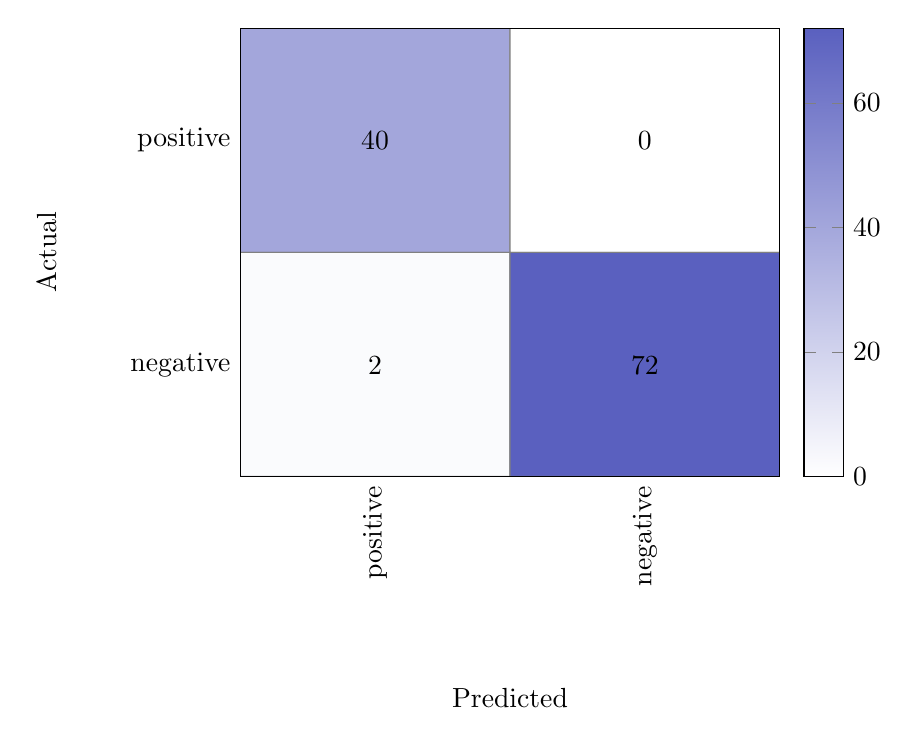
\begin{tikzpicture}
    \begin{axis}[
            colormap={bluewhite}{color=(white) rgb255=(90,96,191)},
            xlabel=Predicted,
            xlabel style={yshift=-30pt},
            ylabel=Actual,
            ylabel style={yshift=20pt},
            xticklabels={positive, negative}, % changed
            xtick={0,...,1}, % changed
            xtick style={draw=none},
            yticklabels={positive, negative}, % changed
            ytick={0,...,1}, % changed
            ytick style={draw=none},
            enlargelimits=false,
            colorbar,
            xticklabel style={
              rotate=90
            },
            nodes near coords={\pgfmathprintnumber\pgfplotspointmeta},
            nodes near coords style={
                yshift=-7pt
            },
        ]
        \addplot[
            matrix plot,
            mesh/cols=2, % changed
            point meta=explicit,draw=gray
        ] table [meta=C] {
            x y C
            0 0 40
            1 0 0

            
            0 1 2
            1 1 72


            
        }; % added every entry where x=4 or y=4
    \end{axis}
\end{tikzpicture}
\caption{Confusion matrix error metrics} \label{ConfusionMatrix}
\end{figure}

Figure \ref{ConfusionMatrix} shows the confusion matrix for the serial code test data. There are 40 true positive, 72 true negative, 2 false positive, and 0 false negative.

\clearpage



\section{Libraires}
OpenMP and CUDA are used to parallelize the serial code for this project. Both libraries are explained in the following section.

\subsection{OpenMP}

The code employs OpenMP, a widely used parallel programming framework, to parallelize the neural network model's forward and backward propagation steps. These steps involve complex computations that can benefit from parallelization, as they can be computationally expensive and time-consuming, especially when dealing with large datasets.

\bigskip 

During forward propagation, the input data is processed through the neural network to calculate the activations of each neuron in the network. The code leverages OpenMP pragmas, which are compiler directives that guide the compiler to generate multi-threaded code. Specifically, the \#\texttt{pragma omp parallel for pragma} is used to parallelize the computation of the weighted sum of inputs, the application of activation functions, and the calculation of the output of each neuron. This pragma distributes the computations across multiple threads, allowing them to work concurrently on different neurons, thereby speeding up the forward propagation process.

\bigskip

Backward propagation involves computing the gradients of the neural network's parameters (e.g., weights and biases) with respect to the loss function, which is essential for updating the parameters during the training process. The code uses OpenMP pragmas to parallelize this step as well. For example, during the calculation of the gradients of the weights and biases, the \#\texttt{pragma omp parallel for pragma} is used to parallelize the computation across multiple threads. This enables concurrent computation of the gradients for different neurons, leading to improved performance.

\bigskip

As multiple threads are involved in parallel computation, proper synchronization mechanisms are necessary to prevent race conditions, which occur when multiple threads access shared data simultaneously and result in unexpected behavior. OpenMP provides synchronization constructs such as critical sections, atomic operations, and locks that can be used to protect shared data. In the code, appropriate synchronization mechanisms, such as critical sections or atomic operations, are used to ensure that the updates to the shared parameters are done correctly and consistently, avoiding any conflicts among threads. By leveraging OpenMP for parallelization, the code can take advantage of multi-core processors' processing power to perform parallel computations, leading to significant performance improvements. Parallelization allows the code to process larger datasets and perform more complex computations in less time, resulting in faster training and prediction times for the neural network model. 



\subsubsection{Forward Propagation}

\begin{lstlisting}[style=CStyle, caption={Forward path openMP of main.c}, label={lst:forwardpathopenMP}]
    // forward pass
    // compute hidden layer activation

    // hidden layer 1
    #pragma omp parallel for num_threads(thread_count)
    for(int j =0; j < numHiddenNodes; j++){
        double activation = hiddenLayerBias[j];

        for(int k = 0; k < numInputs; k++){
            activation += trainingInputs[i][k] * hiddenWeights[k][j];
        }

        hiddenLayer[j] = relu(activation);
    }

    // hidden layer 2
    double activation = 0;
    #pragma omp parallel for reduction(+:activation) num_threads(thread_count)
    for(int j =0; j < numHiddenNodes2; j++){
        activation = hiddenLayerBias2[j];

        for(int k = 0; k < numHiddenNodes; k++){
            activation += hiddenLayer[k] * hiddenWeights2[k][j];
        }

        hiddenLayer2[j] = relu(activation);
    }

    // compute output layer activation
    #pragma omp parallel for reduction(+:activation) num_threads(thread_count)
    for(int j =0; j < numOutputs; j++){
        activation = outputLayerBias[j];

        for(int k = 0; k < numHiddenNodes2; k++){
            activation += hiddenLayer2[k] * outputWeights[k][j];
        }

        outputLayer[j] = sigmoid(activation);
    }
\end{lstlisting}


Listing \ref{lst:forwardpathopenMP} shows part of the forward propagation path of a Deep Neural Network (DNN). The first loop computes the activation of the neurons in the first hidden layer, and it is parallelized using OpenMP's parallel directive. Each thread executes the loop body for a subset of the iterations, with thread-count specifying the number of threads to be used. The second loop computes the activation of the neurons in the second hidden layer, and it is also parallelized using OpenMP's parallel for directive. In addition, the reduction clause is used to sum up the values of the activation variable across threads. This loop body is executed for all iterations by all threads, and the reduction clause ensures that the final value of activation is the sum of the partial values computed by each thread. The third loop computes the activation of the output layer neurons and is similar to the second loop in terms of its use of OpenMP's parallel for and reduction clauses. 


\subsubsection{Backward Propagation}
\begin{lstlisting}[style=CStyle, caption={Backward path openMP of main.c}, label={lst:backwardpathopenMP}]
    // Backpropagation
    // Compute change in output weights
    double deltaOutput[numOutputs];
    #pragma omp parallel for num_threads(thread_count)
    for(int j = 0; j < numOutputs; j++){
        double error = (trainingOutputs[i][j] - outputLayer[j]); // L1
        deltaOutput[j] = error * dSigmoid(outputLayer[j]) ;
    }

    // Compute change in hidden weights (second layer)
    double deltaHidden2[numHiddenNodes2];
    #pragma omp parallel for num_threads(thread_count)
    for(int j = 0; j < numHiddenNodes2; j++){
        double error = 0.0f;
        for(int k = 0; k < numOutputs; k++){
            error += deltaOutput[k] * outputWeights[j][k];
        }
        deltaHidden2[j] = error * dRelu(hiddenLayer[j]);
    }

    // Compute change in hidden weights (first layer)
    double deltaHidden[numHiddenNodes];
    #pragma omp parallel for num_threads(thread_count)
    for(int j = 0; j < numHiddenNodes; j++){
        double error = 0.0f;
        for(int k = 0; k < numHiddenNodes2; k++){
            error += deltaHidden2[k] * hiddenWeights2[j][k];
        }
        deltaHidden[j] = error * dRelu(hiddenLayer2[j]);
    }

    // Apply change in output weights
    #pragma omp parallel for num_threads(thread_count)
    for(int j = 0; j < numOutputs; j++){
        outputLayerBias[j] += deltaOutput[j] * lr;
        for(int k = 0; k < numHiddenNodes2; k++){
            outputWeights[k][j] += hiddenLayer2[k] * deltaOutput[j] * lr;
        }
    }

    // Apply change in second hidden layer weights
    #pragma omp parallel for num_threads(thread_count)
    for(int j = 0; j < numHiddenNodes2; j++){
        hiddenLayerBias[j] += deltaHidden[j] * lr;
        for(int k = 0; k < numHiddenNodes; k++){
            hiddenWeights2[k][j] += hiddenLayer[k] * deltaHidden2[j] * lr;
        }
    }

    // Apply change in first hidden layer weights
    #pragma omp parallel for num_threads(thread_count)
    for(int j = 0; j < numHiddenNodes; j++){
        hiddenLayerBias[j] += deltaHidden[j] * lr;
        for(int k = 0; k < numInputs; k++){
            hiddenWeights[k][j] += trainingInputs[i][k] * deltaHidden[j] * lr;
        }
    }
\end{lstlisting}

Listing \ref{lst:backwardpathopenMP} shows the backward propagation path of a Deep Neural Network using OpenMP. Each of the for loops is parallelized using the pragma statements.  The code starts by computing the change in output weights using the training inputs and outputs. This computation uses the OpenMP parallel construct, which splits the loop iterations across multiple threads. The num\_threads(thread\_count) clause specifies the number of threads to use for the parallel computation, which is set to thread\_count. Next, the code computes the change in hidden weights for the second layer and then the first layer. Again, both of these computations are done in parallel using the parallel construct. After computing the changes in the weights, the code applies them to the network by updating the weights and biases. The updates are done in parallel using the parallel for construct for each weight and bias array.

\subsubsection{Results}
For 4800 inputs, 4800 hidden nodes in both the layers and 1 epoch. The DNN is running for the following time:
Tserial=527.12s
\begin{table}[H]
\centering
\begin{tabular}{|c|c|c|c|c|c|c|c|c|c|}
\hline
 p & 1 & 2 & 4 & 8 & 16 & 32 & 64 & 128 & 256 \\ \hline
 $T_{parallel}$ [s] & 548.5 & 279.1 & 163.3 & 86.6 & 51.13 & 62.71 & 60.23 & 60.36 & 64.84 \\ \hline
\end{tabular}
\caption{Execution times for parallization with openMP} \label{timeopenMP}
\end{table}

\begin{figure}[H]
    \centering
    \includegraphics[width=0.8\textwidth]{Plots/exec_openMP.png}
    \caption{Graph for execution times for parallelization with openMP from Table \ref{timeopenMP}}
    \label{fig:exec_openMP}
\end{figure}

Table \ref{timeopenMP} shows the execution times for parallelization using OpenMP for increasing the number of threads (represented by "p"). The serial execution time is also given as a reference. The parallel execution times decrease as the number of threads increases, indicating that the parallelization is effective. However, the execution time does not continue to decrease at the same rate as the number of threads increases. This is likely due to overhead costs associated with creating and managing threads. There is also a slight increase in execution time when using 16 threads, which could be due to contention for shared resources. Overall, the table suggests that using 8 or 16 threads provides the best balance between performance gains and overhead costs.

\begin{table}[H]
\centering
\begin{tabular}{|c|c|c|c|c|c|c|c|c|c|}
\hline
 p      & 1 & 2 & 4 & 8 & 16 & 32 & 64 & 128 & 256 \\ \hline
 $T_{S}$  & 0.96 & 1.89 & 3.23 & 6.09 & 10.3 & 8.41 & 2.71 & 2.71 & 2.52 \\ \hline
 $T_{E}$  & 0.96 & 0.94 & 0.81 & 0.76 & 0.64 & 0.26 & 0.04 & 1.35 & 0.63 \\ \hline
\end{tabular}
\caption{Speedup and efficiency using OpenMP} \label{speedupefficiencyomp}
\end{table}


\bigskip

Table \ref{speedupefficiencyomp} shows that the speedup increases as the number of processors increases, but with diminishing returns. This is reflected in the decreasing efficiency, which measures the amount of speedup achieved per processor. We can also see that there is a dip in both speedup and efficiency at 32 processors, indicating that this may not be the best number of processors to use for this particular program. Additionally, we can see that the efficiency is quite low for some of the larger numbers of processors, indicating that the parallel implementation may not be very effective beyond a certain number of processors.



\begin{figure}[H]
    \centering
    \includegraphics[width=0.8\textwidth]{Plots/speedup_omp.png}
    \caption{Graph for speedup and efficiency for parallelization with openMP from Table \ref{speedupefficiencyomp}}
    \label{fig:speedup_omp}
\end{figure}

\clearpage

\subsection{CUDA}

The CUDA code uses the parallel processing capability of the GPU to speed up the computations involved in the forward and backward propagation steps of the neural network. These steps can be computationally intensive, especially when dealing with large datasets, making it important to parallelize them.

\bigskip

The forward propagation kernel processes the input data through the neural network to calculate the activations of each neuron in the network. The CUDA code leverages the parallel processing power of the GPU by launching multiple threads to perform the calculations concurrently. Specifically, the \texttt{\_\_global\_\_} keyword indicates that this function is a kernel, which will be executed on the GPU. The \texttt{blockIdx.x} and \texttt{threadIdx.x} variables are used to compute each thread's unique index. The \texttt{\_\_syncthreads()} function synchronizes threads and ensures correct data dependency.

\bigskip

The backward propagation kernel computes the gradients of the neural network's parameters with respect to the loss function. This step is critical for updating the parameters during the training process. The backward propagation is not parallelized.

\subsubsection{Forward Propagation}
\begin{lstlisting}[style=CStyle, caption={Forward path CUDA of main.c}, label = {lst:ForwardpathCodeCUDA}]
// Forward propagation kernel
__global__ void forward_kernel(double* X, double* W1, double* W2, double* W3, double* b1, double* b2, double* b3, double* hidden1, double* hidden2, double* output) {
    int tid = blockIdx.x * blockDim.x + threadIdx.x;

    if (tid < HIDDEN_SIZE) {
        double sum = 0.0;
        for (int j = 0; j < INPUT_SIZE; j++) {
            sum += X[j] * W1[j * HIDDEN_SIZE + tid];
        }
        hidden1[tid] = relu(sum + b1[tid]);
    }

    __syncthreads();

    if (tid < HIDDEN_SIZE) {
        double sum = 0.0;
        for (int i = 0; i < HIDDEN_SIZE; i++) {
            sum += hidden1[i] * W2[i * HIDDEN_SIZE + tid];
        }
        hidden2[tid] = relu(sum + b2[tid]);
    }

    __syncthreads();

    if (tid == 0) {
        double sum = 0.0;
        for (int i = 0; i < HIDDEN_SIZE; i++) {
            sum += hidden2[i] * W3[i];
        }
        *output = sigmoid(sum + b3[0]);
    }
}
\end{lstlisting}

Listing \ref{lst:ForwardpathCodeCUDA} shows the code of a CUDA kernel function performing forward propagation in a neural network with two hidden layers. The kernel takes as input the weights and biases of the network (W1, W2, W3, b1, b2, and b3), the input data X, and preallocated arrays for the hidden layers (hidden1 and hidden2) and output (output). The kernel uses parallel processing to compute the activations of the hidden layers and the output in a batched fashion. Specifically, it divides the input data and preallocated arrays into thread blocks, each containing a group of threads. Each thread is responsible for computing the activations of a specific neuron in the hidden layers or the output layer. The kernel starts by computing the activations of the neurons in the first hidden layer, computes the dot product, applies ReLU, and stores the resulting activations in the hidden1 array. This process is repeated for hidded2 and output array. The output array calculation here uses the Sigmoid function. 

\subsubsection{Backward Propagation}
\begin{lstlisting}[style=CStyle, caption={Backward CUDA path of main.c}, label={lst:backwardpathCodeCUDA}]
__global__ void backward_kernel(double* X, double* W1, double* W2, double* W3, double* b1, double* b2, double* b3, double* hidden1, double* hidden2, double* output, double target) {
    int tid = blockIdx.x * blockDim.x + threadIdx.x;

    if (tid == 0) {
        // calculate output weight
        double d_output = (*output - target) * dSigmoid(*output);

        // calculate hidden 2 weight
        double d_hidden2[HIDDEN_SIZE];
        for (int i = 0; i < HIDDEN_SIZE; i++) {
            d_hidden2[i] = dRelu(hidden2[i]) * W3[i] * d_output;
        }
        
        // calculate hidden 1 weight
        double d_hidden1[HIDDEN_SIZE];
        for (int i = 0; i < HIDDEN_SIZE; i++) {
            double sum = 0.0;
            for (int j = 0; j < HIDDEN_SIZE; j++) {
                sum += W3[j * HIDDEN_SIZE + i] * d_hidden2[j];
            }
            d_hidden1[i] = dRelu(hidden1[i]) * sum;
        }

        // update hidden weights 1 & bias
        for (int i = 0; i < HIDDEN_SIZE; i++) {
            for (int j = 0; j < INPUT_SIZE; j++) {
                W1[j * HIDDEN_SIZE + i] -= LEARNING_RATE * X[j] * d_hidden1[i];
            }
            b1[i] -= LEARNING_RATE * d_hidden1[i];
        }

        // update hidden weights 2 & bias
        for (int i = 0; i < HIDDEN_SIZE; i++) {
            for (int j = 0; j < HIDDEN_SIZE; j++) {
                W2[j * HIDDEN_SIZE + i] -= LEARNING_RATE * hidden1[i] * d_hidden2[j];
            }
            b2[i] -= LEARNING_RATE * d_hidden2[i];
        }

        // update output weights & bias
        for (int i = 0; i < HIDDEN_SIZE; i++) {
            W3[i] -= LEARNING_RATE * hidden2[i] * d_output;
        }
        b3[0] -= LEARNING_RATE * d_output;
    }
}
\end{lstlisting}

Listing \ref{lst:backwardpathCodeCUDA} is a CUDA kernel for backpropagation in a neural network, but it is not parallelized. The kernel takes in the weights and biases for the network, as well as the input data and target output. The goal of backpropagation is to adjust the weights and biases of the network in order to reduce the error between the predicted output and the target output. The first part of the backward propagation kernel computes the gradient of the weights connecting the second hidden layer to the output layer. Thread zero computes the derivative of the Sigmoid function applied to the output, multiplied by the error between the output and the target output. This value represents the rate of change of the output with respect to the input, which is used to update the weights. 

\bigskip

The second part of the backward propagation kernel computes the gradient of the weights connecting the first hidden layer to the second hidden layer. Thread zero computes the derivative of the ReLU function applied to the activations in the second hidden layer, multiplied by the sum of the products of the weights connecting the second hidden layer to the output layer and the gradients computed in the previous step for each neuron in the second hidden layer. 

\bigskip

The final part of the backward propagation kernel computes the gradient of the weights connecting the input layer to the first hidden layer. Thread zero computes the derivative of the ReLU function applied to the activations in the first hidden layer, multiplied by the sum of the products of the weights connecting the first hidden layer to the second hidden layer and the gradients computed in the previous step, for each neuron in the first hidden layer. The updated weights and biases are then computed using these gradients and the learning rate.

\subsubsection{Results}

The CUDA implementation of our DNN has presented several challenges, particularly with regard to memory management, so we ended up using only 570 inputs instead of 4800. The runtime error we are currently facing is related to illegal memory access, which we have not been able to resolve within the given time frame. Our limited knowledge and lack of practical experience with parallelization are also hindering our progress. Unfortunately, we were not able to devote enough time to this task, as we only became familiar with the technique a few days ago and had a limited understanding of it. As a result, we conducted a series of runs with different numbers of threads, and the outcomes are summarized below.

\bigskip

For 570 inputs, the DNN is running for the following time:
Tserial=71.24 seconds
\begin{table}[H]
\centering
\begin{tabular}{|c|c|c|c|c|c|c|c|c|c|}
\hline
 p & 1 & 2 & 4 & 8 & 16 & 32 & 64 & 128 & 256 \\ \hline
 $T_{parallel}$ [s] & 71.24 & 71.23 & 71.24 & 71.13 & 71 & 70.73 & 70.19 & 69.22 & 68.21 \\ \hline
\end{tabular}
\caption{Execution times for parallelization with CUDA} \label{timeCUDA}
\end{table}

\begin{figure}[H]
    \centering
    \includegraphics[width=0.7\textwidth]{Plots/time_CUDA.png}
    \caption{Graph for execution times for parallelization with CUDA from Table \ref{timeCUDA}}
    \label{fig:exec_CUDA}
\end{figure}

\begin{table}[H]
\centering
\begin{tabular}{|c|c|c|c|c|c|c|c|c|c|}
\hline
p & 1 & 2 & 4 & 8 & 16 & 32 & 64 & 128 & 256 \\ \hline
$T_S$ & 1.00 & 1.00 & 1.00 & 1.00 & 1.00 & 1.01 & 1.01 & 1.03 & 1.04 \\ \hline
$T_E$ & 1.00 & 0.50 & 0.25 & 0.13 & 0.06 & 0.03 & 0.02 & 0.01 & 0.00 \\ \hline
\end{tabular}
\caption{Speedup and efficiency for parallelization with CUDA} \label{speedupefficiencycuda}
\end{table}


\begin{figure}[H]
    \centering
    \includegraphics[width=0.7\textwidth]{Plots/speedup_cuda.png}
    \caption{Graph for speedup and efficiency for parallelization with CUDA from Table \ref{speedupefficiencycuda}}
    \label{fig:speedup_cuda}
\end{figure}


Table \ref{timeCUDA} shows the execution times of the parallelization with CUDA for different numbers of threads ($p$). The execution time remains almost constant, around 71 seconds, with only a slight improvement as the number of processors increases. This indicates that the parallelization is not effective in reducing the overall execution time. We suspect that this is because of we are not able to run with a higher number of inputs, so the overhead is balancing out the parallelization. One thing to note here is that we are not parallelizing the backpropagation. As seen in Table \ref{speedupefficiencycuda}, the speedup is almost 1 for all numbers of processors, indicating that the parallelization does not provide any significant speedup. The efficiency decreases as the number of processors increases, which suggests that the parallelization is not well-suited for the given problem (given the number of inputs). To improve parallelization, we can optimize the kernel by using shared memory to cache the inputs and weights that are reused within a block. 

\bigskip

Better parallelization can also be achieved by parallelizing the backward propagation. Optimizing memory usage with techniques such as  memory coalescing, using shared memory, and reducing global memory access can also increase overall performance. There are also specialized libraries like cuDNN, which provide optimized CUDA implementations of commonly used deep learning operations such as convolution and pooling.




%\begin{table}[H]
%\centering
%\begin{tabular}{|c|c|c|c|c|c|c|c|c|c|}
%\hline
%$p$ & 1 & 2 & 4 & 8 & 16 & 32 & 64 & 128 & 256 \\ \hline
%$T_S$ & 6502 & 21797 & 21867 & 21678 & 20570 & 21678 & 8394 & 6394 & 6408 \\ \hline
%T_E$ & 6502.5 & 10898.5 & 5466.8 & 2709.7 & 1285.6 & 678.6 & 131.1 & 49.9 & 25.2 \\ \hline
%\end{tabular}
%\caption{Speedup and efficiency for parallelization with Cuda ($T_{serial}$ = 527.12 seconds)} \label{speedupefficiencycudawithothertime}
%\end{table}

\clearpage

\section{How to run the code}
You can find all the deliverables in the finalProject folder on tuckoo. For your convenience, we have included a README.md file in the directories for DeepNeuralNetwork, OpenMP, and CUDA. These files provide instructions on how to run the code.


\section{Comparison (Literature)}

\subsection{OpenMP: comparision}

Times:
1 epoch, 4800 cols, 1 rows, only sigmoid activation, 2 hidden layers
serial:
0.49s

\begin{table}[H]
\centering
\begin{tabular}{|c|c|c|c|c|c|c|c|c|c|}
\hline
 p & 1 & 2 & 4 & 8 & 16 & 32 & 64 & 128 & 256 \\ \hline
 $T_{parallel}$ & 0.49 & 0.25 & 0.16 & 0.09 & 0.05 & 0.06 & 0.05 & 0.05 & 0.06  \\ \hline
\end{tabular}
\caption{Execution times for parallelization with openMP with only Forward Propagation} \label{timeopenMPcomparision}
\end{table}

\begin{figure}[H]
    \centering
    \includegraphics[width=0.7\textwidth]{Plots/exec_openMP_comp.png}
    \caption{Graph for execution times for parallelization with openMP from Table \ref{timeopenMPcomparision}}
    \label{fig:exec_openMP_comp}
\end{figure}

\begin{table}[H]
\centering
\begin{tabular}{|c|c|c|c|c|c|c|c|c|c|}
\hline
 p      & 1 & 2 & 4 & 8 & 16 & 32 & 64 & 128 & 256 \\ \hline
 $T_{S}$ & 1 & 1.96 & 3.06 & 5.44 & 9.80 & 8.17 & 9.80 & 9.80 & 8.17  \\ \hline
 $T_{E}$  & 1 & 0.98 & 0.76 & 0.68 & 0.61 & 0.25 & 0.15 & 0.07 & 0.03 \\ \hline
\end{tabular}
\caption{Speedup and efficiency for parallelization with openMP} \label{speedupompcomp}
\end{table}


Table \ref{speedupompcomp} shows the speedup and efficiency achieved through parallelization with OpenMP for varying numbers of threads. As expected, the speedup increases with the number of threads until it reaches its peak and then starts to decrease. The peak speedup is achieved with 16 threads, where the program runs 9.8 times faster than the serial version. The efficiency, which is the speedup normalized by the number of threads, starts to decrease rapidly when the number of threads exceeds 16, indicating diminishing returns from additional threads due to overheads associated with parallelization. Notably, the program's execution time is not consistently decreasing as we increase the number of threads, which suggests that there may be some contention or load imbalance in the parallelization that is hindering the performance.

\begin{figure}[H]
    \centering
    \includegraphics[width=0.7\textwidth]{Plots/speedup_omp_comp.png}
    \caption{Graph for speedup and efficiency for parallelization with openMP from Table \ref{speedupompcomp}}
    \label{fig:speedup_omp_comp}
\end{figure}


\bigskip 

\begin{table}[H]
\centering
\begin{tabular}{|c|c|c|c|c|c|c|c|c|c|}
\hline
 p & 1 & 2 & 4 & 8 & 16 & 32 & 64 & 128 & 256 \\ \hline
 $T_{parallel}$ & 0.000309 & 0.011793 & 0.024327 & 0.032643 & 0.022938 & 0.032647 & 0.032645 & 0.033629 & 0.032897  \\ \hline
\end{tabular}
\caption{Execution times (in seconds) for parallelization with Orlandi's OpenMP with only Forward Propagation} \label{timeOrlandiOpenMPcomparision}
\end{table}

\begin{table}[H]
\centering
\begin{tabular}{|c|c|c|c|c|c|c|c|c|c|}
\hline
 p      & 1 & 2 & 4 & 8 & 16 & 32 & 64 & 128 & 256 \\ \hline
 $T_{S}$ & 1.000 & 0.026 & 0.013 & 0.009 & 0.013 & 0.009 & 0.009 & 0.009 & 0.009 \\ \hline
 $T_{E}$  & 1.00000 & 0.01310 & 0.00318 & 0.00118 & 0.00084 & 0.00030 & 0.00015 & 0.00007 & 0.00004 \\ \hline
\end{tabular}
\caption{Speedup and efficiency for parallelization with openMP} \label{speedupompcomporlandi}
\end{table}

Table \ref{timeOrlandiOpenMPcomparision} suggests that Orlandi's parallelization does not work for small numbers of rows, as prescribed by his code. The times were very fast; however, the code does not scale as the number of threads increases. As shown by Table \ref{speedupompcomporlandi}, there are little gains in speedup and efficiency as more threads are added. These minimal marginal gains are likely due to the limited number of rows that are processed by Orlandi's OpenMP implementation.


\begin{figure}[H]
    \centering
    \includegraphics[width=0.7\textwidth]{Plots/comparision_openMP_time.png}
    \caption{Orlandi's parallelization from table \ref{timeOrlandiOpenMPcomparision}}
    \label{fig:speedupomporlandi}
\end{figure}

\begin{figure}[H]
    \centering
    \includegraphics[width=0.7\textwidth]{Plots/time_comp_openMP.png}
    \caption{Orlandi's parallelization vs. our Neural Network from table \ref{timeOrlandiOpenMPcomparision}}
    \label{fig:timecomparision}
\end{figure}

Figure \ref{fig:timecomparision} shows that our DNN takes longer to train compared to Orlandi's; nevertheless, we are able to parallelize the process using OpenMP efficiently.  

\begin{figure}[H]
    \centering
    \includegraphics[width=0.7\textwidth]{Plots/speedupcompopenmp.png}
    \caption{Orlandi's parallelization vs. our Neural Network (Speedup and Efficiency)}
    \label{fig:speedupcomparision}
\end{figure}

Figure \ref{fig:speedupcomparision}, we see that though our neural network takes longer to train compared to that of Orlandi's, we can reach higher speedups, and our code is more efficient comparatively. In the figure green line is not seen clearly as it is behind the $T_s-Orlandi$. 

\subsection{CUDA: comparision}
Times:
1 epoch, 4800 cols, 1 row, only Sigmoid activation, 2 hidden layers
serial: 574.82ms

\begin{table}[H]
\centering
\begin{tabular}{|c|c|c|c|c|c|c|c|c|c|}
\hline
 p & 1 & 2 & 4 & 8 & 16 & 32 & 64 & 128 & 256 \\ \hline
 $T_{parallel}$ & 687.95 & 511.46 & 467.03 & 426.02 & 402.94 & 340.41 & 332.02 & 330.53 & 329.83  \\ \hline
\end{tabular}
\caption{Execution times for parallelization with CUDA with only Forward Propagation} \label{exec_CUDA_comp}
\end{table}

\begin{table}[H]
\centering
\begin{tabular}{|c|c|c|c|c|c|c|c|c|c|}
\hline
p         & 1     & 2     & 4     & 8     & 16    & 32    & 64    & 128   & 256 \\ \hline
 $T_{S}$  & 0.836 & 1.124 & 1.231 & 1.349 & 1.427 & 1.689 & 1.731 & 1.739 & 1.743 \\ \hline
 $T_{E}$  & 0.836 & 0.562 & 0.308 & 0.169 & 0.089 & 0.053 & 0.027 & 0.014 & 0.007 \\ \hline
 \end{tabular}
\caption{Speedup and efficiency for parallelization with CUDA} \label{speedup_CUDA_comp}
\end{table}

As shown in the Table \ref{speedup_CUDA_comp}, there was a slight speedup by using more threads. However, the forward propagation is much faster using CUDA than OpenMP, with it completing in milliseconds rather than seconds. The problem shows very weak scalability, so we would expect better efficiencies with a larger amount of inputs but not much of an increase with each additional thread. As discussed in the literature review, we were unable to run the CUDA comparison code in Tuckoo as the code does not recognize the internal Tuckoo architecture.


\begin{figure}[H]
    \centering
    \includegraphics[width=0.7\textwidth]{Plots/exec_CUDA_comp.png}
    \caption{Graph for execution times for parallelization with CUDA from Table \ref{exec_CUDA_comp}}
    \label{fig:execCUDAcomp}
\end{figure}


\begin{figure}[H]
    \centering
    \includegraphics[width=0.7\textwidth]{Plots/speedup_CUDA_comp.png}
    \caption{Graph for speedup and efficiency for parallelization with CUDA from Table \ref{speedup_CUDA_comp}}
    \label{fig:speedupCUDAcomp}
\end{figure}


\clearpage

\section{Conclusion}


The project shows that parallelizing a neural network model requires careful planning to avoid incorrect information being read by processes and threads due to race conditions but is possible and scalable. The parallelization of forward propagation is possible due to its need of dot product multiplication for each layer. However, as shown in our code, each layer needs to read the results of the previous layer, so the problem proves to be weakly scalable.

\bigskip

A similar parallelization occurs with backward propagation, where the gradient of the cost function is calculated by a dot product, and the gradient descent is applied as well by a dot product. However, each layer depends on the previous layer's calculations, so the parallelization is limited and weakly scalable.


\bigskip 

Based on the results presented in Tables \ref{timeCUDA} and \ref{timeopenMP}, we can conclude that the parallelization of the neural network model using CUDA is not very effective in reducing the overall execution time. This is likely due to the overhead associated with parallelization and the relatively small number of input data points used in the experiment. However, parallelization using OpenMP is effective in reducing execution time, with a significant speedup achieved using 8 or 16 threads. The efficiency decreases as the number of processors increases, suggesting that the parallelization is not well-suited for larger numbers of processors. We couldn't compare OpenMP and CUDA directly with each other due to different parallelization techniques and different input sizes. 

\bigskip

In general, parallelizing a neural network model is advantageous when dealing with a large amount of input data and a large number of neurons per layer. However, the scalability of a neural network is weak in terms of the number of layers, limiting the potential gains from parallelization. To improve the scalability, one could consider optimizing the parallelization strategy, such as reducing the dependencies between layers or implementing techniques like pipelining. Overall, our experiments provide insights into the strengths and limitations of different parallelization techniques for neural networks and suggest avenues for further optimization.


\section{Discussion}

As a showcase of the parallelization of neural networks, we have expanded upon Orlandi's forward propagation parallelization and have implemented a fully functioning parallelized neural network. Although our forward propagation times do not match that of Orlandi's due to time constraints, ours fulfills the goal of creating one of practical use. 

\bigskip

In future iterations of this project, a forward propagation method that comes close to matching the speed of Orlandi's method would be ideal in optimizing our neural network, especially our CUDA code. We would also need access to a system that can run Orlandi's CUDA parallelization code to compare ours to his.

\bigskip

We had a difficult time implementing the CUDA coding due to our inexperience of the system as the deadline approached. With more experience in CUDA, future iterations will be able to expand upon our more basic code. We were unable to parallelize and had issues with memory management with our forward propagation and thus had to limit the number of inputs to 570 and could not parallelize the backward propagation. We believe these issues are due to not having enough time to learn CUDA and needing to implement an arguably more complex parallelization. Since we only parallelized the inner loops of the forward propagation, future editions could parallelize the outer loop since each forward propagation epoch does not depend on the previous epoch. However, this presents problems with incorporating backward propagation.

\bigskip

Finally, as with any software project, future iterations could benefit from additional testing and optimization to ensure optimal performance and accuracy. Additional testing could include training the neural network on larger datasets or using more complex models to assess the scalability and performance of the parallelization techniques implemented. Overall, we are proud of the performance of our neural network model and have a deeper understanding of how neural networks and parallelization work.


\section{Division of Work}
Equal work was performed by all project members.

% include bibliography
\bibliography{sample} 
\bibliographystyle{IEEEtran}


\end{document}
